\section{Scanchain Silicon Results}
\label{sec:scan_chain_res}

TT02 chips were received in October 2023, \(11\) months after the chips were submitted for manufacture on Efabless chipIgnite 2211Q.
The chips were tested for the first time in public on a livestream\cite{siliconalive}.
The chain was validated, and a few of the designs were shown to be working.

\begin{figure}[htp]
\centering
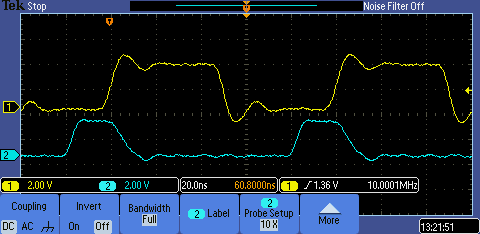
\includegraphics[width=\columnwidth]{./Figs/tt02_clock_out.png}
\caption{Measurement from TT02 silicon, with input clock in yellow and the distorted output clock in blue.}
\label{fig:TT02_clock_out}
\end{figure}

In the following days another \(30\) designs were tested and shown to be working.

After measuring the clock asymmetry (Fig.~\ref{fig:TT02_clock_out}) and maximum frequency it was decided to run the production boards with a \(20MHz\) oscillator, resulting in a \(10MHz\) scan chain.

Some designs didn’t function as expected, which in most cases was due to faults in the submitted design.

As well as \(82\) Verilog designs, \(64\) used the Wokwi graphical editor, \(6\) used alternative HDLs like VHDL, Amaranth\cite{amaranth} and Chisel\cite{chisel}.
Some Wokwi designs using combinational logic in clock paths (Fig.~\ref{fig:failed_design_comb_logic}) worked in simulation but failed in hardware.
This was due to the lack of timing data in the simulation, and wasn’t detected by STA because the clock paths were not known.
A detailed analysis has yet to be carried out.
The addition of SR flops to Wokwi will help to alleviate this, as well as the start of an ERC check.

\begin{figure}[htp]
\centering
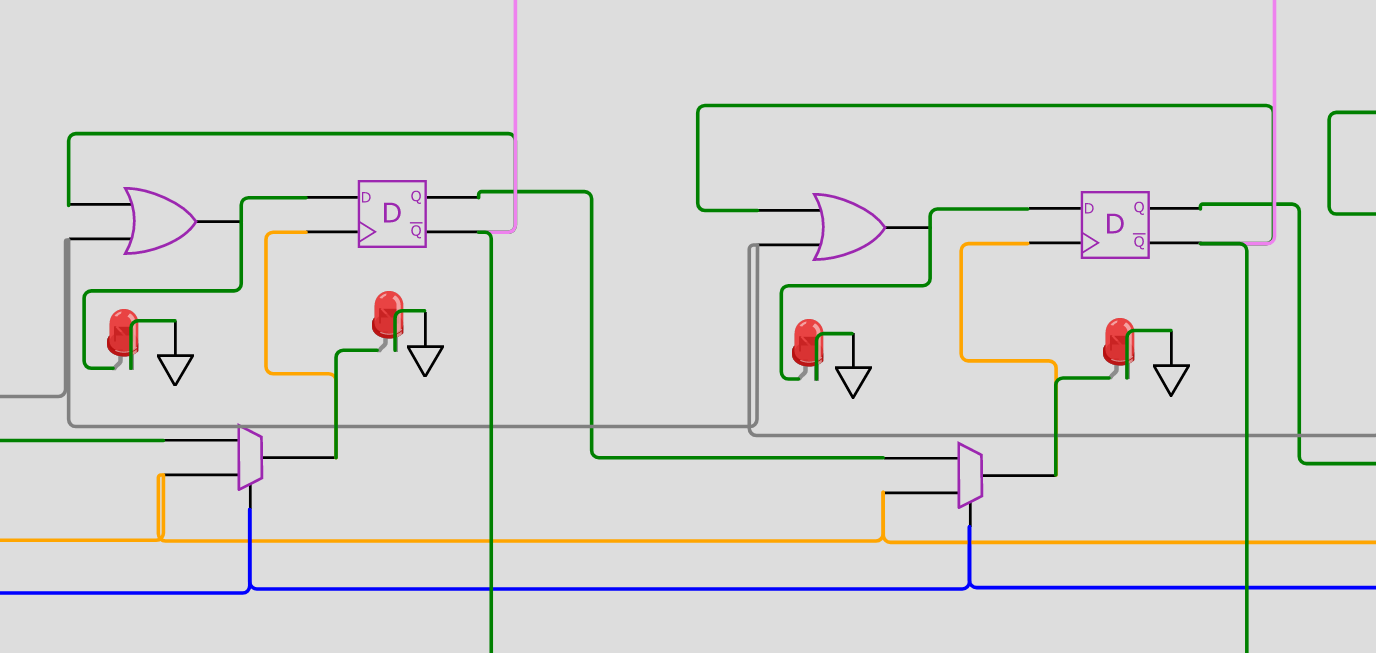
\includegraphics[width=\columnwidth]{./Figs/wokwi mux clock logic.png}
\caption{Combination logic in the clock path of one of the failed designs.}
\label{fig:failed_design_comb_logic}
\end{figure}

At the time of writing, PCBs are in production and are expected to ship to customers by the end of January 2024.

TinyTapeout 3 silicon was received in January 2024, and the updated scanchain shows a more symmetric (Fig.~\ref{fig:TT03_silicon_measurement}) output clock at the end of the chain. This will allow a faster scanchain clock, resulting in a faster update frequency.

\begin{figure}[htp]
\centering
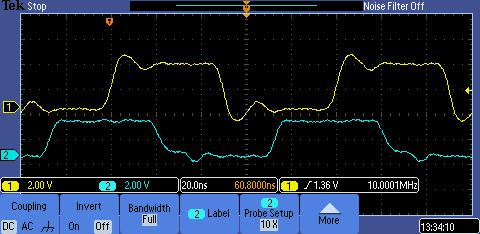
\includegraphics[width=\columnwidth]{./Figs/tt03_clock_out.png}
\caption{Measurement from TT03 silicon.}
\label{fig:TT03_silicon_measurement}
\end{figure}
